\clearpage
\newpage
\subsubsection{Estensione D: Gestione degli Errori in Fase di Pubblicazione}

Nel caso in cui, al momento della pubblicazione dell'annuncio immobiliare, il sistema rilevi errori in alcuni campi del form, viene attivato un meccanismo di gestione degli errori progettato per minimizzare la frustrazione dell’utente e facilitare la correzione delle informazioni errate.

\newline
\subsubsection{Feedback Visivo e Navigazione Intelligente}
Per evitare che l’utente debba individuare manualmente i campi errati, il sistema implementa un’animazione che lo riporta automaticamente al primo step contenente errori. Inoltre, sopra il titolo dello step viene visualizzato un messaggio chiaro che segnala la presenza di dati non corretti. Questo messaggio include un riepilogo dei campi che necessitano di correzione, garantendo così un'immediata comprensione del problema senza dover scorrere l’intero form.

\subsubsection{Evidenziazione degli Errori nei Campi del Form}
I campi contenenti errori vengono evidenziati attraverso i seguenti accorgimenti visivi:
\begin{itemize}
    \item Il bordo del campo assume un colore rosso evidente, attirando immediatamente l’attenzione dell’utente.
    \item Al di sotto del campo appare un messaggio testuale che spiega chiaramente la natura dell’errore (ad esempio, "Inserire un numero valido per il prezzo" o "Il titolo dell’annuncio non può essere vuoto").
\end{itemize}

Questa strategia segue i principi di 	extit{error prevention} e 	extit{error recovery} proposti da Nielsen \cite{nielsen1995}, permettendo all’utente di comprendere e correggere rapidamente gli errori.

\newline
\subsubsection{Indicazione degli Step con Errori}
Per garantire una visione d'insieme immediata dello stato del form, il sistema modifica dinamicamente il colore dei riquadri degli step nel percorso di navigazione:
\begin{itemize}
    \item Gli step senza errori mantengono il colore verde, confermando all’utente che le informazioni inserite sono corrette.
    \item Gli step contenenti errori cambiano colore dal verde al rosso, segnalando visivamente dove è necessario intervenire, senza bisogno di ulteriori spiegazioni testuali.
\end{itemize}

Questa soluzione si basa sui principi dell’	extit{immediate feedback} e dell’	extit{error mapping} \cite{shneiderman2004}, riducendo il carico cognitivo e migliorando l’usabilità complessiva del sistema.
\newline
\subsubsection{Esperienza Utente e Riduzione della Frustrazione}
L’implementazione di questi meccanismi mira a ottimizzare l’esperienza dell’utente durante la compilazione del form, minimizzando la frustrazione derivante dalla correzione degli errori. La combinazione di feedback visivo, animazioni intuitive e segnalazioni mirate permette un’interazione fluida e priva di ostacoli, in linea con le best practice in ambito UX.


\begin{figure}[ht]
    \centering
    \begin{tikzpicture}[node distance=1.5cm and 1cm, auto]
        % Nodo per immagine 1 con didascalia sotto
        \node (img1) {
            \begin{tabular}{c}
                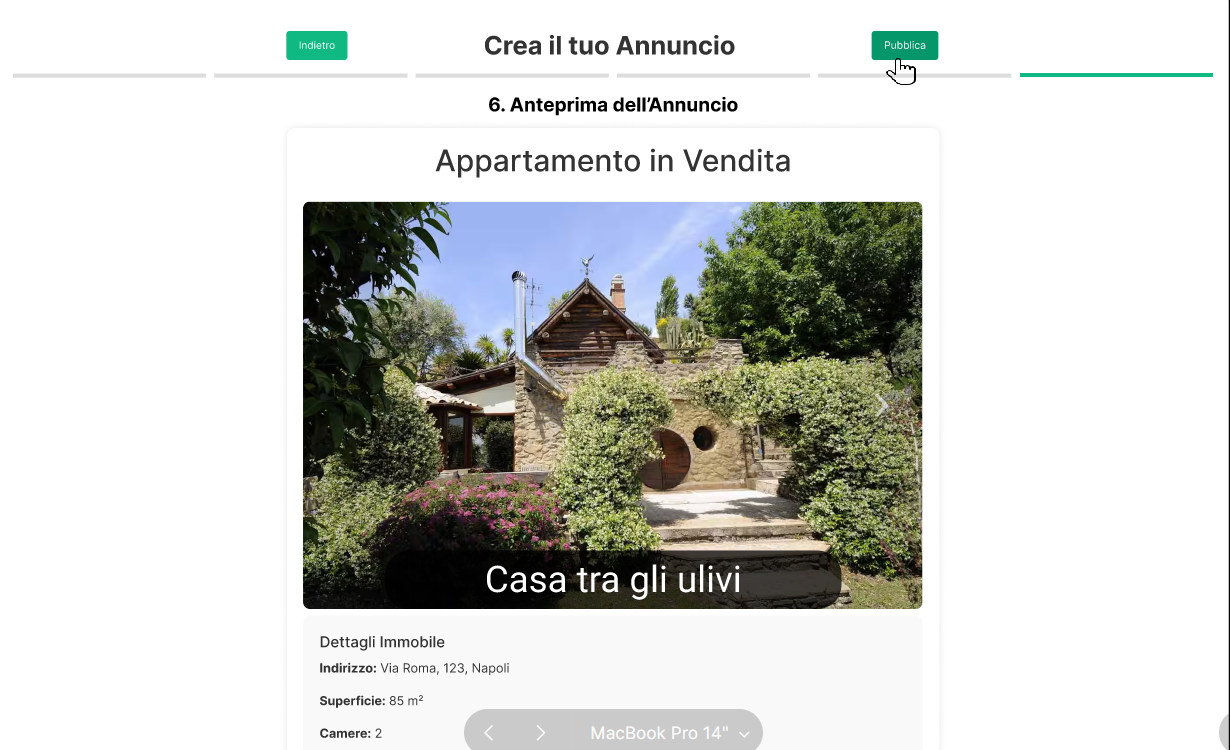
\includegraphics[width=0.7\textwidth]{Immagini/Mockup/aggiungi annuncio/estensione D/step1.png} \\
                click pubblica nuovo annuncio
            \end{tabular}
        };
        
        % Nodo per immagine 2 con didascalia sotto, posizionato a destra di img1
        \node (img2) [below=of img1] {
            \begin{tabular}{c}
                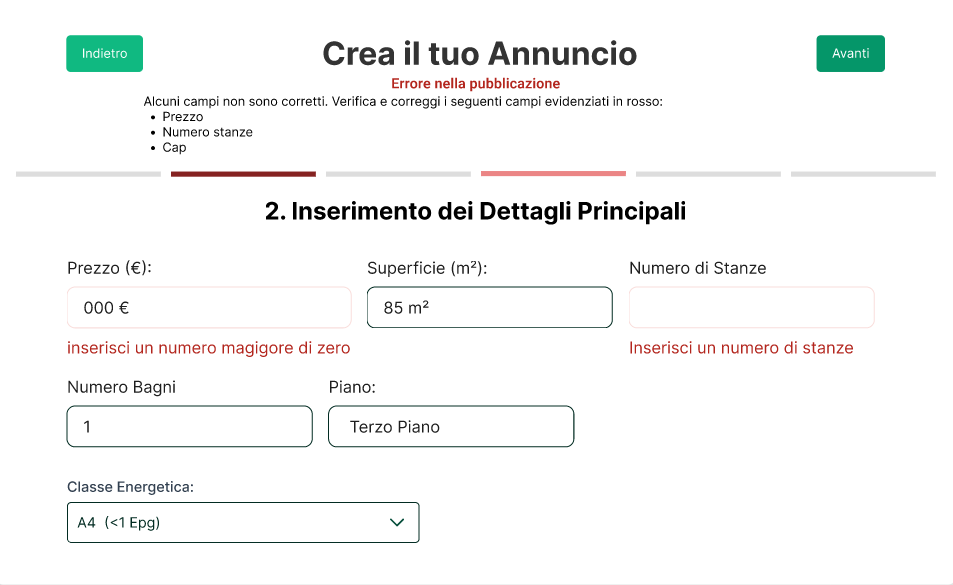
\includegraphics[width=0.7\textwidth]{Immagini/Mockup/aggiungi annuncio/estensione D/step3.png} \\
                Cockburn: extension D.10
            \end{tabular}
        };
        
        
        % Disegna le frecce
        \draw[->, thick] (img1) -- (img2);
      
    \end{tikzpicture}
    \caption{Mockup: estensione D della tabella di Cockburn del caso d'uso nuovo annuncio}
    \label{fig:tikz_flow}
\end{figure}

\newpage